\documentclass[]{article}
\usepackage{lmodern}
\usepackage{amssymb,amsmath}
\usepackage{ifxetex,ifluatex}
\usepackage{fixltx2e} % provides \textsubscript
\ifnum 0\ifxetex 1\fi\ifluatex 1\fi=0 % if pdftex
  \usepackage[T1]{fontenc}
  \usepackage[utf8]{inputenc}
\else % if luatex or xelatex
  \ifxetex
    \usepackage{mathspec}
  \else
    \usepackage{fontspec}
  \fi
  \defaultfontfeatures{Ligatures=TeX,Scale=MatchLowercase}
\fi
% use upquote if available, for straight quotes in verbatim environments
\IfFileExists{upquote.sty}{\usepackage{upquote}}{}
% use microtype if available
\IfFileExists{microtype.sty}{%
\usepackage{microtype}
\UseMicrotypeSet[protrusion]{basicmath} % disable protrusion for tt fonts
}{}
\usepackage[margin=1in]{geometry}
\usepackage{hyperref}
\hypersetup{unicode=true,
            pdftitle={HW 7 - KELLY SCOTT SIMS},
            pdfborder={0 0 0},
            breaklinks=true}
\urlstyle{same}  % don't use monospace font for urls
\usepackage{color}
\usepackage{fancyvrb}
\newcommand{\VerbBar}{|}
\newcommand{\VERB}{\Verb[commandchars=\\\{\}]}
\DefineVerbatimEnvironment{Highlighting}{Verbatim}{commandchars=\\\{\}}
% Add ',fontsize=\small' for more characters per line
\usepackage{framed}
\definecolor{shadecolor}{RGB}{248,248,248}
\newenvironment{Shaded}{\begin{snugshade}}{\end{snugshade}}
\newcommand{\KeywordTok}[1]{\textcolor[rgb]{0.13,0.29,0.53}{\textbf{#1}}}
\newcommand{\DataTypeTok}[1]{\textcolor[rgb]{0.13,0.29,0.53}{#1}}
\newcommand{\DecValTok}[1]{\textcolor[rgb]{0.00,0.00,0.81}{#1}}
\newcommand{\BaseNTok}[1]{\textcolor[rgb]{0.00,0.00,0.81}{#1}}
\newcommand{\FloatTok}[1]{\textcolor[rgb]{0.00,0.00,0.81}{#1}}
\newcommand{\ConstantTok}[1]{\textcolor[rgb]{0.00,0.00,0.00}{#1}}
\newcommand{\CharTok}[1]{\textcolor[rgb]{0.31,0.60,0.02}{#1}}
\newcommand{\SpecialCharTok}[1]{\textcolor[rgb]{0.00,0.00,0.00}{#1}}
\newcommand{\StringTok}[1]{\textcolor[rgb]{0.31,0.60,0.02}{#1}}
\newcommand{\VerbatimStringTok}[1]{\textcolor[rgb]{0.31,0.60,0.02}{#1}}
\newcommand{\SpecialStringTok}[1]{\textcolor[rgb]{0.31,0.60,0.02}{#1}}
\newcommand{\ImportTok}[1]{#1}
\newcommand{\CommentTok}[1]{\textcolor[rgb]{0.56,0.35,0.01}{\textit{#1}}}
\newcommand{\DocumentationTok}[1]{\textcolor[rgb]{0.56,0.35,0.01}{\textbf{\textit{#1}}}}
\newcommand{\AnnotationTok}[1]{\textcolor[rgb]{0.56,0.35,0.01}{\textbf{\textit{#1}}}}
\newcommand{\CommentVarTok}[1]{\textcolor[rgb]{0.56,0.35,0.01}{\textbf{\textit{#1}}}}
\newcommand{\OtherTok}[1]{\textcolor[rgb]{0.56,0.35,0.01}{#1}}
\newcommand{\FunctionTok}[1]{\textcolor[rgb]{0.00,0.00,0.00}{#1}}
\newcommand{\VariableTok}[1]{\textcolor[rgb]{0.00,0.00,0.00}{#1}}
\newcommand{\ControlFlowTok}[1]{\textcolor[rgb]{0.13,0.29,0.53}{\textbf{#1}}}
\newcommand{\OperatorTok}[1]{\textcolor[rgb]{0.81,0.36,0.00}{\textbf{#1}}}
\newcommand{\BuiltInTok}[1]{#1}
\newcommand{\ExtensionTok}[1]{#1}
\newcommand{\PreprocessorTok}[1]{\textcolor[rgb]{0.56,0.35,0.01}{\textit{#1}}}
\newcommand{\AttributeTok}[1]{\textcolor[rgb]{0.77,0.63,0.00}{#1}}
\newcommand{\RegionMarkerTok}[1]{#1}
\newcommand{\InformationTok}[1]{\textcolor[rgb]{0.56,0.35,0.01}{\textbf{\textit{#1}}}}
\newcommand{\WarningTok}[1]{\textcolor[rgb]{0.56,0.35,0.01}{\textbf{\textit{#1}}}}
\newcommand{\AlertTok}[1]{\textcolor[rgb]{0.94,0.16,0.16}{#1}}
\newcommand{\ErrorTok}[1]{\textcolor[rgb]{0.64,0.00,0.00}{\textbf{#1}}}
\newcommand{\NormalTok}[1]{#1}
\usepackage{graphicx,grffile}
\makeatletter
\def\maxwidth{\ifdim\Gin@nat@width>\linewidth\linewidth\else\Gin@nat@width\fi}
\def\maxheight{\ifdim\Gin@nat@height>\textheight\textheight\else\Gin@nat@height\fi}
\makeatother
% Scale images if necessary, so that they will not overflow the page
% margins by default, and it is still possible to overwrite the defaults
% using explicit options in \includegraphics[width, height, ...]{}
\setkeys{Gin}{width=\maxwidth,height=\maxheight,keepaspectratio}
\IfFileExists{parskip.sty}{%
\usepackage{parskip}
}{% else
\setlength{\parindent}{0pt}
\setlength{\parskip}{6pt plus 2pt minus 1pt}
}
\setlength{\emergencystretch}{3em}  % prevent overfull lines
\providecommand{\tightlist}{%
  \setlength{\itemsep}{0pt}\setlength{\parskip}{0pt}}
\setcounter{secnumdepth}{0}
% Redefines (sub)paragraphs to behave more like sections
\ifx\paragraph\undefined\else
\let\oldparagraph\paragraph
\renewcommand{\paragraph}[1]{\oldparagraph{#1}\mbox{}}
\fi
\ifx\subparagraph\undefined\else
\let\oldsubparagraph\subparagraph
\renewcommand{\subparagraph}[1]{\oldsubparagraph{#1}\mbox{}}
\fi

%%% Use protect on footnotes to avoid problems with footnotes in titles
\let\rmarkdownfootnote\footnote%
\def\footnote{\protect\rmarkdownfootnote}

%%% Change title format to be more compact
\usepackage{titling}

% Create subtitle command for use in maketitle
\newcommand{\subtitle}[1]{
  \posttitle{
    \begin{center}\large#1\end{center}
    }
}

\setlength{\droptitle}{-2em}

  \title{HW 7 - KELLY ``SCOTT'' SIMS}
    \pretitle{\vspace{\droptitle}\centering\huge}
  \posttitle{\par}
    \author{}
    \preauthor{}\postauthor{}
    \date{}
    \predate{}\postdate{}
  

\begin{document}
\maketitle

Using the same crime data set uscrime.txt as in Questions 8.2 and 9.1,
find the best model you can using (a) a regression tree model, and (b) a
random forest model. In R, you can use the tree package or the rpart
package, and the randomForest package. For each model, describe one or
two qualitative takeaways you get from analyzing the results (i.e.,
don't just stop when you have a good model, but interpret it too).

\subsubsection{Load Libraries}\label{load-libraries}

\begin{Shaded}
\begin{Highlighting}[]
\KeywordTok{library}\NormalTok{(rsample)     }\CommentTok{# data splitting }
\end{Highlighting}
\end{Shaded}

\begin{verbatim}
## Loading required package: tidyr
\end{verbatim}

\begin{Shaded}
\begin{Highlighting}[]
\KeywordTok{library}\NormalTok{(dplyr)       }\CommentTok{# data wrangling}
\end{Highlighting}
\end{Shaded}

\begin{verbatim}
## 
## Attaching package: 'dplyr'
\end{verbatim}

\begin{verbatim}
## The following objects are masked from 'package:stats':
## 
##     filter, lag
\end{verbatim}

\begin{verbatim}
## The following objects are masked from 'package:base':
## 
##     intersect, setdiff, setequal, union
\end{verbatim}

\begin{Shaded}
\begin{Highlighting}[]
\KeywordTok{library}\NormalTok{(rpart)       }\CommentTok{# performing regression trees}
\KeywordTok{library}\NormalTok{(rpart.plot)  }\CommentTok{# plotting regression trees}
\KeywordTok{library}\NormalTok{(randomForest)}
\end{Highlighting}
\end{Shaded}

\begin{verbatim}
## randomForest 4.6-14
\end{verbatim}

\begin{verbatim}
## Type rfNews() to see new features/changes/bug fixes.
\end{verbatim}

\begin{verbatim}
## 
## Attaching package: 'randomForest'
\end{verbatim}

\begin{verbatim}
## The following object is masked from 'package:dplyr':
## 
##     combine
\end{verbatim}

\begin{Shaded}
\begin{Highlighting}[]
\KeywordTok{library}\NormalTok{(h2o)}
\end{Highlighting}
\end{Shaded}

\begin{verbatim}
## 
## ----------------------------------------------------------------------
## 
## Your next step is to start H2O:
##     > h2o.init()
## 
## For H2O package documentation, ask for help:
##     > ??h2o
## 
## After starting H2O, you can use the Web UI at http://localhost:54321
## For more information visit http://docs.h2o.ai
## 
## ----------------------------------------------------------------------
\end{verbatim}

\begin{verbatim}
## 
## Attaching package: 'h2o'
\end{verbatim}

\begin{verbatim}
## The following objects are masked from 'package:stats':
## 
##     cor, sd, var
\end{verbatim}

\begin{verbatim}
## The following objects are masked from 'package:base':
## 
##     &&, %*%, %in%, ||, apply, as.factor, as.numeric, colnames,
##     colnames<-, ifelse, is.character, is.factor, is.numeric, log,
##     log10, log1p, log2, round, signif, trunc
\end{verbatim}

\begin{Shaded}
\begin{Highlighting}[]
\KeywordTok{library}\NormalTok{(ggplot2)}
\end{Highlighting}
\end{Shaded}

\begin{verbatim}
## 
## Attaching package: 'ggplot2'
\end{verbatim}

\begin{verbatim}
## The following object is masked from 'package:randomForest':
## 
##     margin
\end{verbatim}

\begin{Shaded}
\begin{Highlighting}[]
\KeywordTok{library}\NormalTok{(caTools)}
\KeywordTok{library}\NormalTok{(caret)}
\end{Highlighting}
\end{Shaded}

\begin{verbatim}
## Loading required package: lattice
\end{verbatim}

\begin{Shaded}
\begin{Highlighting}[]
\KeywordTok{library}\NormalTok{(pROC)}
\end{Highlighting}
\end{Shaded}

\begin{verbatim}
## Type 'citation("pROC")' for a citation.
\end{verbatim}

\begin{verbatim}
## 
## Attaching package: 'pROC'
\end{verbatim}

\begin{verbatim}
## The following object is masked from 'package:h2o':
## 
##     var
\end{verbatim}

\begin{verbatim}
## The following objects are masked from 'package:stats':
## 
##     cov, smooth, var
\end{verbatim}

\subsubsection{Load the data and
inspect}\label{load-the-data-and-inspect}

\begin{Shaded}
\begin{Highlighting}[]
\NormalTok{data <-}\StringTok{ }\KeywordTok{read.table}\NormalTok{(}\StringTok{'uscrime.txt'}\NormalTok{, }\DataTypeTok{header =} \OtherTok{TRUE}\NormalTok{, }\DataTypeTok{stringsAsFactors =} \OtherTok{FALSE}\NormalTok{)}
\CommentTok{#Separate independent and dependent variables just in case}
\NormalTok{Y =}\StringTok{ }\KeywordTok{as.data.frame}\NormalTok{((data[,}\DecValTok{16}\NormalTok{]))}
\NormalTok{X =}\StringTok{ }\KeywordTok{as.data.frame}\NormalTok{(data[,}\DecValTok{1}\OperatorTok{:}\DecValTok{15}\NormalTok{])}
\KeywordTok{head}\NormalTok{(data)}
\end{Highlighting}
\end{Shaded}

\begin{verbatim}
##      M So   Ed  Po1  Po2    LF   M.F Pop   NW    U1  U2 Wealth Ineq
## 1 15.1  1  9.1  5.8  5.6 0.510  95.0  33 30.1 0.108 4.1   3940 26.1
## 2 14.3  0 11.3 10.3  9.5 0.583 101.2  13 10.2 0.096 3.6   5570 19.4
## 3 14.2  1  8.9  4.5  4.4 0.533  96.9  18 21.9 0.094 3.3   3180 25.0
## 4 13.6  0 12.1 14.9 14.1 0.577  99.4 157  8.0 0.102 3.9   6730 16.7
## 5 14.1  0 12.1 10.9 10.1 0.591  98.5  18  3.0 0.091 2.0   5780 17.4
## 6 12.1  0 11.0 11.8 11.5 0.547  96.4  25  4.4 0.084 2.9   6890 12.6
##       Prob    Time Crime
## 1 0.084602 26.2011   791
## 2 0.029599 25.2999  1635
## 3 0.083401 24.3006   578
## 4 0.015801 29.9012  1969
## 5 0.041399 21.2998  1234
## 6 0.034201 20.9995   682
\end{verbatim}

\subsection{\# CART}\label{cart}

With regressions trees, there's no need to scale the data before
constructing a model. See quote below as noted from
stats.stackexchange.com

\begin{quote}
``Standardization does not add or subtract information contained in a
given variable and does not distort its relationship to a target
variable. For example, if you had a variable''age" which was a predictor
for ``purchase car''. By changing age to (age - mean / sd ) is not going
to change its relationship to purchase car, it merely maps it to a new
space. When CART looks for the best splits, it going to use entropy or
gini to calculate information gain, this is not dependent on the scale
of your predictor variable, rather on the resultant purity of the
variable ``purchase car''."
\end{quote}

\subsubsection{Build the CART model}\label{build-the-cart-model}

\begin{Shaded}
\begin{Highlighting}[]
\NormalTok{cart_model <-}\StringTok{ }\KeywordTok{rpart}\NormalTok{(}
  \DataTypeTok{formula =}\NormalTok{ Crime }\OperatorTok{~}\StringTok{ }\NormalTok{.,}
  \DataTypeTok{data    =}\NormalTok{ data,}
  \DataTypeTok{method  =} \StringTok{"anova"}
\NormalTok{  )}

\KeywordTok{summary}\NormalTok{(cart_model)}
\end{Highlighting}
\end{Shaded}

\begin{verbatim}
## Call:
## rpart(formula = Crime ~ ., data = data, method = "anova")
##   n= 47 
## 
##           CP nsplit rel error    xerror      xstd
## 1 0.36296293      0 1.0000000 1.0374862 0.2616639
## 2 0.14814320      1 0.6370371 0.8234956 0.1971550
## 3 0.05173165      2 0.4888939 0.9945709 0.2088903
## 4 0.01000000      3 0.4371622 1.0017542 0.2096042
## 
## Variable importance
##    Po1    Po2 Wealth   Ineq   Prob      M     NW    Pop   Time     Ed 
##     17     17     11     11     10     10      9      5      4      4 
##     LF     So 
##      1      1 
## 
## Node number 1: 47 observations,    complexity param=0.3629629
##   mean=905.0851, MSE=146402.7 
##   left son=2 (23 obs) right son=3 (24 obs)
##   Primary splits:
##       Po1    < 7.65      to the left,  improve=0.3629629, (0 missing)
##       Po2    < 7.2       to the left,  improve=0.3629629, (0 missing)
##       Prob   < 0.0418485 to the right, improve=0.3217700, (0 missing)
##       NW     < 7.65      to the left,  improve=0.2356621, (0 missing)
##       Wealth < 6240      to the left,  improve=0.2002403, (0 missing)
##   Surrogate splits:
##       Po2    < 7.2       to the left,  agree=1.000, adj=1.000, (0 split)
##       Wealth < 5330      to the left,  agree=0.830, adj=0.652, (0 split)
##       Prob   < 0.043598  to the right, agree=0.809, adj=0.609, (0 split)
##       M      < 13.25     to the right, agree=0.745, adj=0.478, (0 split)
##       Ineq   < 17.15     to the right, agree=0.745, adj=0.478, (0 split)
## 
## Node number 2: 23 observations,    complexity param=0.05173165
##   mean=669.6087, MSE=33880.15 
##   left son=4 (12 obs) right son=5 (11 obs)
##   Primary splits:
##       Pop < 22.5      to the left,  improve=0.4568043, (0 missing)
##       M   < 14.5      to the left,  improve=0.3931567, (0 missing)
##       NW  < 5.4       to the left,  improve=0.3184074, (0 missing)
##       Po1 < 5.75      to the left,  improve=0.2310098, (0 missing)
##       U1  < 0.093     to the right, improve=0.2119062, (0 missing)
##   Surrogate splits:
##       NW   < 5.4       to the left,  agree=0.826, adj=0.636, (0 split)
##       M    < 14.5      to the left,  agree=0.783, adj=0.545, (0 split)
##       Time < 22.30055  to the left,  agree=0.783, adj=0.545, (0 split)
##       So   < 0.5       to the left,  agree=0.739, adj=0.455, (0 split)
##       Ed   < 10.85     to the right, agree=0.739, adj=0.455, (0 split)
## 
## Node number 3: 24 observations,    complexity param=0.1481432
##   mean=1130.75, MSE=150173.4 
##   left son=6 (10 obs) right son=7 (14 obs)
##   Primary splits:
##       NW   < 7.65      to the left,  improve=0.2828293, (0 missing)
##       M    < 13.05     to the left,  improve=0.2714159, (0 missing)
##       Time < 21.9001   to the left,  improve=0.2060170, (0 missing)
##       M.F  < 99.2      to the left,  improve=0.1703438, (0 missing)
##       Po1  < 10.75     to the left,  improve=0.1659433, (0 missing)
##   Surrogate splits:
##       Ed   < 11.45     to the right, agree=0.750, adj=0.4, (0 split)
##       Ineq < 16.25     to the left,  agree=0.750, adj=0.4, (0 split)
##       Time < 21.9001   to the left,  agree=0.750, adj=0.4, (0 split)
##       Pop  < 30        to the left,  agree=0.708, adj=0.3, (0 split)
##       LF   < 0.5885    to the right, agree=0.667, adj=0.2, (0 split)
## 
## Node number 4: 12 observations
##   mean=550.5, MSE=20317.58 
## 
## Node number 5: 11 observations
##   mean=799.5455, MSE=16315.52 
## 
## Node number 6: 10 observations
##   mean=886.9, MSE=55757.49 
## 
## Node number 7: 14 observations
##   mean=1304.929, MSE=144801.8
\end{verbatim}

The summary statistic above explains steps of the splits. For example,
we start with n = 47 observations at the root node (very beginning) and
the first variable we split on (the first variable that optimizes a
reduction in SSE) is Po1. Node \#2 has 23 observations and is split on
Pop. Opposite of that node is Node \#3 being split on NW. We could
continue to analyze these superfluous statistics, but it is much easier
to just visualize the tree itself.

\subsection{\#Note:}\label{note}

At the very top of the summary statistics above, there is a cp table
which lists the 4 nodes after 3 splits. For the 3rd split, we see the
xerror term is \emph{1.005}. This is what we will be trying to imporve
upon

\subsubsection{Plot the Regression Tree}\label{plot-the-regression-tree}

\begin{Shaded}
\begin{Highlighting}[]
\KeywordTok{rpart.plot}\NormalTok{(cart_model)}
\end{Highlighting}
\end{Shaded}

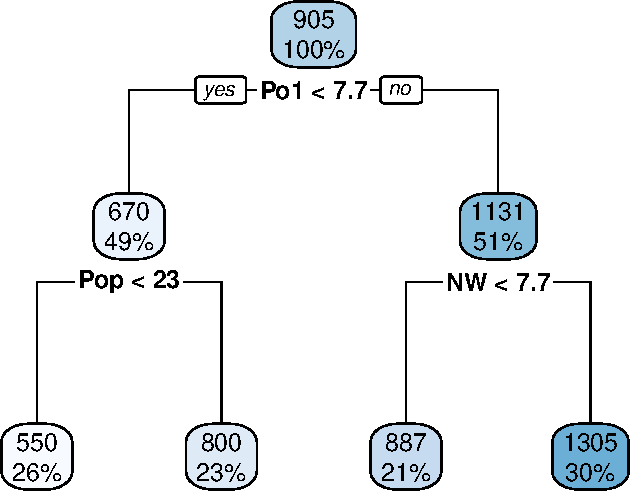
\includegraphics{HW7_files/figure-latex/unnamed-chunk-4-1.pdf} This
visualization makes it easier to see that in the initial model, there
were only three splits performed. These splits coincide with what was
stated above, Po1 being the most important factor followed by Pop and NW
respectively. But if three features are being split upon, what about the
other 12 features in the model? According to the post below, rpart is
doing the following behind the scenes

\begin{quote}
Behind the scenes rpart is automatically applying a range of cost
complexity (αlpha) values to prune the tree. To compare the error for
each αlpha value, rpart performs a 10-fold cross validation so that the
error associated with a given αlpha value is computed on the hold-out
validation data.
\end{quote}

In this example, we find diminishing returns for the 4 terminal nodes as
seen blelow. The y-axis is the cross validation error. The lower x-axis
is cost complexity parameter (alpha), and the upper x-axis is the number
of terminal nodes. The complexity parameter (cp) is used to control the
size of the decision tree and to select the optimal tree size. If the
cost of adding another variable to the decision tree from the current
node is above the value of cp, then tree building does not continue. We
could also say that tree construction does not continue unless it would
decrease the overall lack of fit by a factor of cp.

\begin{Shaded}
\begin{Highlighting}[]
\KeywordTok{plotcp}\NormalTok{(cart_model)}
\end{Highlighting}
\end{Shaded}

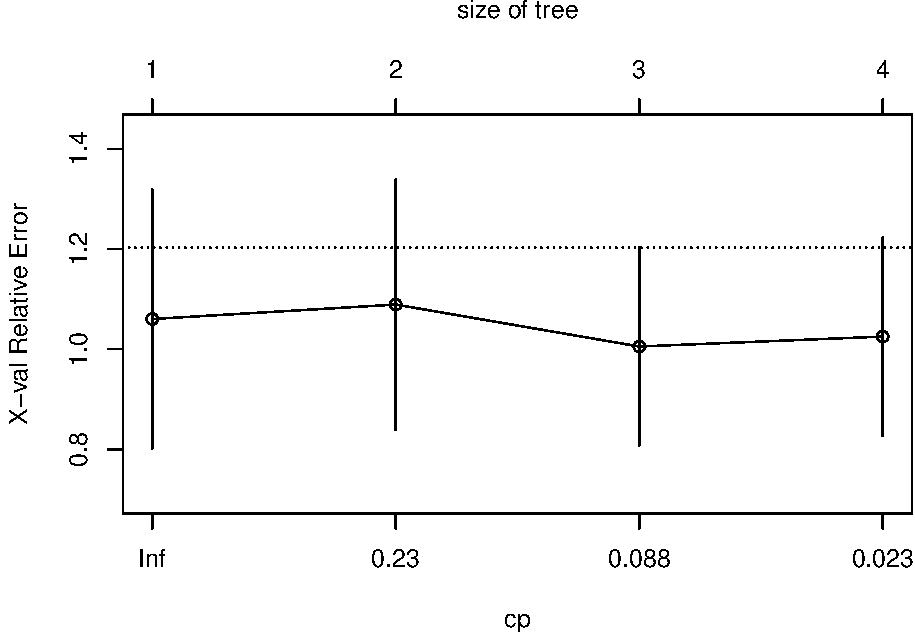
\includegraphics{HW7_files/figure-latex/unnamed-chunk-5-1.pdf}

\subsubsection{Tuning the model with
Gridsearch}\label{tuning-the-model-with-gridsearch}

In addition to the cost complexity parameter, it is also common to tune:

\begin{enumerate}
\def\labelenumi{\arabic{enumi}.}
\tightlist
\item
  minsplit: the minimum number of data points required to attempt a
  split before it is forced to create a terminal node. The default is
  20. Making this smaller allows for terminal nodes that may contain
  only a handful of observations to create the predicted value.
\item
  maxdepth: the maximum number of internal nodes between the root node
  and the terminal nodes. The default is 30, which is quite liberal and
  allows for fairly large trees to be built.
\end{enumerate}

To perform a grid search we first create our hyperparameter grid. In
this example, I search a range of minsplit from 1-20 and vary maxdepth
from 2-15. This gives 280 different hyperparameter combinations to try.

\begin{Shaded}
\begin{Highlighting}[]
\NormalTok{hyper_grid <-}\StringTok{ }\KeywordTok{expand.grid}\NormalTok{(}
  \DataTypeTok{minsplit =} \KeywordTok{seq}\NormalTok{(}\DecValTok{1}\NormalTok{, }\DecValTok{20}\NormalTok{, }\DecValTok{1}\NormalTok{),}
  \DataTypeTok{maxdepth =} \KeywordTok{seq}\NormalTok{(}\DecValTok{2}\NormalTok{, }\DecValTok{15}\NormalTok{, }\DecValTok{1}\NormalTok{)}
\NormalTok{)}

\KeywordTok{head}\NormalTok{(hyper_grid)}
\end{Highlighting}
\end{Shaded}

\begin{verbatim}
##   minsplit maxdepth
## 1        1        2
## 2        2        2
## 3        3        2
## 4        4        2
## 5        5        2
## 6        6        2
\end{verbatim}

\begin{Shaded}
\begin{Highlighting}[]
\KeywordTok{length}\NormalTok{(hyper_grid[,}\DecValTok{1}\NormalTok{])}
\end{Highlighting}
\end{Shaded}

\begin{verbatim}
## [1] 280
\end{verbatim}

\section{Iterate through the hypergrid creating a model for each
combination}\label{iterate-through-the-hypergrid-creating-a-model-for-each-combination}

We will store the resulting model in a list called models. We will use
this list of models to extract the best one

\begin{Shaded}
\begin{Highlighting}[]
\NormalTok{models <-}\StringTok{ }\KeywordTok{list}\NormalTok{()}

\ControlFlowTok{for}\NormalTok{ (i }\ControlFlowTok{in} \DecValTok{1}\OperatorTok{:}\KeywordTok{nrow}\NormalTok{(hyper_grid)) \{}
  
  \CommentTok{# get minsplit, maxdepth values at row i}
\NormalTok{  minsplit <-}\StringTok{ }\NormalTok{hyper_grid}\OperatorTok{$}\NormalTok{minsplit[i]}
\NormalTok{  maxdepth <-}\StringTok{ }\NormalTok{hyper_grid}\OperatorTok{$}\NormalTok{maxdepth[i]}

  \CommentTok{# train a model and store in the list}
\NormalTok{  models[[i]] <-}\StringTok{ }\KeywordTok{rpart}\NormalTok{(}
    \DataTypeTok{formula =}\NormalTok{ Crime }\OperatorTok{~}\StringTok{ }\NormalTok{.,}
    \DataTypeTok{data    =}\NormalTok{ data,}
    \DataTypeTok{method  =} \StringTok{"anova"}\NormalTok{,}
    \DataTypeTok{control =} \KeywordTok{list}\NormalTok{(}\DataTypeTok{minsplit =}\NormalTok{ minsplit, }\DataTypeTok{maxdepth =}\NormalTok{ maxdepth)}
\NormalTok{    )}
\NormalTok{\}}
\end{Highlighting}
\end{Shaded}

\section{Extract the best performing models, and their subsequent
hyperparameters}\label{extract-the-best-performing-models-and-their-subsequent-hyperparameters}

Next, from each model, we will extract the lowest \textbf{xerror} and
the lowest \textbf{cp} value for each model, and append those values to
the hypergrid next to their subseqent hyperparameters. We will then sort
the hypergrid by lowest error and pick the best performing model.

\begin{Shaded}
\begin{Highlighting}[]
\CommentTok{# function to get optimal cp}
\NormalTok{get_cp <-}\StringTok{ }\ControlFlowTok{function}\NormalTok{(x) \{}
\NormalTok{  min    <-}\StringTok{ }\KeywordTok{which.min}\NormalTok{(x}\OperatorTok{$}\NormalTok{cptable[, }\StringTok{"xerror"}\NormalTok{])}
\NormalTok{  cp <-}\StringTok{ }\NormalTok{x}\OperatorTok{$}\NormalTok{cptable[min, }\StringTok{"CP"}\NormalTok{] }
\NormalTok{\}}

\CommentTok{# function to get minimum error}
\NormalTok{get_min_error <-}\StringTok{ }\ControlFlowTok{function}\NormalTok{(x) \{}
\NormalTok{  min    <-}\StringTok{ }\KeywordTok{which.min}\NormalTok{(x}\OperatorTok{$}\NormalTok{cptable[, }\StringTok{"xerror"}\NormalTok{])}
\NormalTok{  xerror <-}\StringTok{ }\NormalTok{x}\OperatorTok{$}\NormalTok{cptable[min, }\StringTok{"xerror"}\NormalTok{] }
\NormalTok{\}}

\NormalTok{hyper_grid }\OperatorTok
\StringTok{  }\KeywordTok{mutate}\NormalTok{(}
    \DataTypeTok{cp    =}\NormalTok{ purrr}\OperatorTok{::}\KeywordTok{map_dbl}\NormalTok{(models, get_cp),}
    \DataTypeTok{error =}\NormalTok{ purrr}\OperatorTok{::}\KeywordTok{map_dbl}\NormalTok{(models, get_min_error)}
\NormalTok{    ) }\OperatorTok
\StringTok{  }\KeywordTok{arrange}\NormalTok{(error) }\OperatorTok
\StringTok{  }\KeywordTok{top_n}\NormalTok{(}\OperatorTok{-}\DecValTok{5}\NormalTok{, }\DataTypeTok{wt =}\NormalTok{ error)}
\end{Highlighting}
\end{Shaded}

\begin{verbatim}
##   minsplit maxdepth   cp     error
## 1        6       13 0.01 0.6444917
## 2       16        4 0.01 0.6544624
## 3       10        7 0.01 0.6880056
## 4        1       10 0.01 0.7194721
## 5        8        9 0.01 0.7217574
\end{verbatim}

We Can see above that the best performing model was one that has a
minsplit of 8, maxdepth of 9 and a cp of 0.01. Let's build this model
and visualize the resulting tree

\section{Best Model}\label{best-model}

\begin{Shaded}
\begin{Highlighting}[]
\NormalTok{optimal_tree <-}\StringTok{ }\KeywordTok{rpart}\NormalTok{(}
    \DataTypeTok{formula =}\NormalTok{ Crime }\OperatorTok{~}\StringTok{ }\NormalTok{.,}
    \DataTypeTok{data    =}\NormalTok{ data,}
    \DataTypeTok{method  =} \StringTok{"anova"}\NormalTok{,}
    \DataTypeTok{control =} \KeywordTok{list}\NormalTok{(}\DataTypeTok{minsplit =} \DecValTok{8}\NormalTok{, }\DataTypeTok{maxdepth =} \DecValTok{9}\NormalTok{, }\DataTypeTok{cp =} \FloatTok{0.01}\NormalTok{)}
\NormalTok{    )}

\KeywordTok{rpart.plot}\NormalTok{(optimal_tree)}
\end{Highlighting}
\end{Shaded}

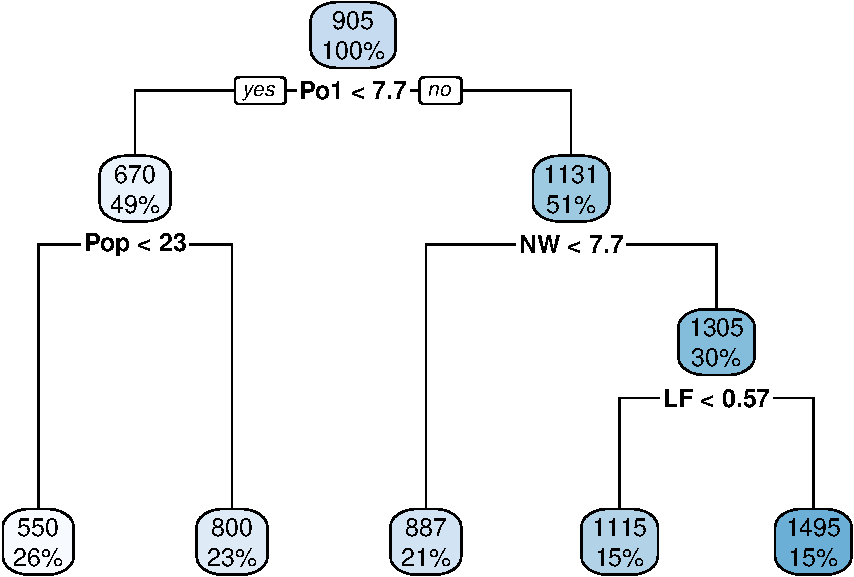
\includegraphics{HW7_files/figure-latex/unnamed-chunk-9-1.pdf}

So here we have the best tuned model. We can see that it just added one
more split from the original model. At the leafs, we can see that there
is 26\% of the data at a Crime rate average of 550, 23\% at a crime rate
average of 800, etc etc. Let's use last weaks ``new unseen data'' and
make a prediction with this model

\subsubsection{Prediction}\label{prediction}

\begin{Shaded}
\begin{Highlighting}[]
\NormalTok{new.data <-}\StringTok{ }\KeywordTok{data.frame}\NormalTok{(}\StringTok{"M"}\NormalTok{=}\StringTok{ }\DecValTok{14}\NormalTok{,}
\StringTok{"So"}\NormalTok{ =}\StringTok{ }\DecValTok{0}\NormalTok{,}
\StringTok{"Ed"}\NormalTok{ =}\StringTok{ }\DecValTok{10}\NormalTok{,}
\StringTok{"Po1"}\NormalTok{ =}\StringTok{ }\DecValTok{12}\NormalTok{,}
\StringTok{"Po2"}\NormalTok{ =}\StringTok{ }\FloatTok{15.5}\NormalTok{,}
\StringTok{"LF"}\NormalTok{ =}\StringTok{ }\NormalTok{.}\DecValTok{640}\NormalTok{,}
\StringTok{"M.F"}\NormalTok{ =}\StringTok{ }\DecValTok{94}\NormalTok{,}
\StringTok{"Pop"}\NormalTok{ =}\StringTok{ }\DecValTok{150}\NormalTok{,}
\StringTok{"NW"}\NormalTok{ =}\StringTok{ }\FloatTok{1.1}\NormalTok{,}
\StringTok{"U1"}\NormalTok{ =}\StringTok{ }\NormalTok{.}\DecValTok{120}\NormalTok{,}
\StringTok{"U2"}\NormalTok{ =}\StringTok{ }\FloatTok{3.6}\NormalTok{,}
\StringTok{"Wealth"}\NormalTok{ =}\StringTok{ }\DecValTok{3200}\NormalTok{,}
\StringTok{"Ineq"}\NormalTok{ =}\StringTok{ }\FloatTok{20.1}\NormalTok{,}
\StringTok{"Prob"}\NormalTok{ =}\StringTok{ }\NormalTok{.}\DecValTok{04}\NormalTok{,}
\StringTok{"Time"}\NormalTok{ =}\StringTok{ }\DecValTok{39}\NormalTok{)}

\KeywordTok{predict}\NormalTok{(optimal_tree, }\DataTypeTok{newdata =}\NormalTok{ new.data)}
\end{Highlighting}
\end{Shaded}

\begin{verbatim}
##     1 
## 886.9
\end{verbatim}

*\textbf{Analysis} We can see that the predicted crime average is 887.
This seems lower than what other models had been predicting in weeks
past. If you trace the regression tree, we can see exactly where the
model divered from expectations. Po1 for the new data is greater than
7.7, so we go to the right side of the tree. Next, we can see that NW is
less than the constraint 7.7, so this moves of to the left of that node,
bringing us to 887. Had it not been for that one lower value, we can see
on the right side of that split, our data is larger than 0.57 for LF,
and that would have brought us around the crime average we have been
seeing, 1495.

\subsection{\# RANDOM FOREST}\label{random-forest}

\begin{Shaded}
\begin{Highlighting}[]
\KeywordTok{set.seed}\NormalTok{(}\DecValTok{42}\NormalTok{)}

\NormalTok{RF_model <-}\StringTok{ }\KeywordTok{randomForest}\NormalTok{(}
  \DataTypeTok{formula =}\NormalTok{ Crime }\OperatorTok{~}\StringTok{ }\NormalTok{.,}
  \DataTypeTok{data    =}\NormalTok{ data}
\NormalTok{)}

\KeywordTok{plot}\NormalTok{(RF_model, }\DataTypeTok{main =} \StringTok{'Random Forest Model'}\NormalTok{)}
\end{Highlighting}
\end{Shaded}

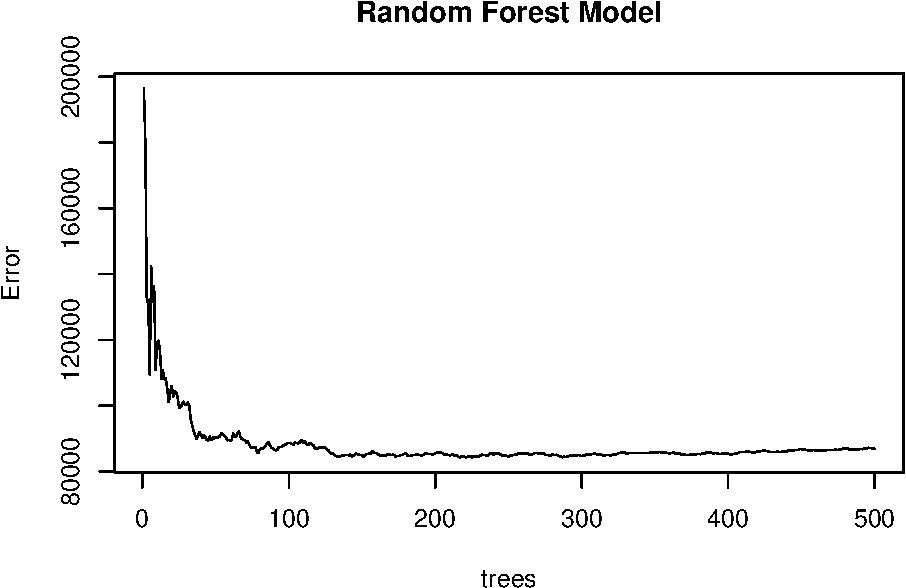
\includegraphics{HW7_files/figure-latex/unnamed-chunk-11-1.pdf}

\begin{Shaded}
\begin{Highlighting}[]
\CommentTok{# number of trees with lowest MSE}
\KeywordTok{which.min}\NormalTok{(RF_model}\OperatorTok{$}\NormalTok{mse)}
\end{Highlighting}
\end{Shaded}

\begin{verbatim}
## [1] 225
\end{verbatim}

\begin{Shaded}
\begin{Highlighting}[]
\CommentTok{# RMSE of this optimal random forest}
\KeywordTok{sqrt}\NormalTok{(RF_model}\OperatorTok{$}\NormalTok{mse[}\KeywordTok{which.min}\NormalTok{(RF_model}\OperatorTok{$}\NormalTok{mse)])}
\end{Highlighting}
\end{Shaded}

\begin{verbatim}
## [1] 290.168
\end{verbatim}

In the plot above we can see the model that produces the lowest (best)
error has about 225 Trees. It's RMSE is 290. After that, the graph
flattens out without much of any improvement. randomForest allows the
use of crossvalidation in order to train a model as well

\subsubsection{Cross Validation}\label{cross-validation}

\subsubsection{Note - the following example is one adapted from an
online source. It is not my original
code}\label{note---the-following-example-is-one-adapted-from-an-online-source.-it-is-not-my-original-code}

\begin{Shaded}
\begin{Highlighting}[]
\KeywordTok{set.seed}\NormalTok{(}\DecValTok{24}\NormalTok{)}
\NormalTok{valid_split <-}\StringTok{ }\KeywordTok{initial_split}\NormalTok{(data, .}\DecValTok{8}\NormalTok{)}

\CommentTok{# training data}
\NormalTok{train <-}\StringTok{ }\KeywordTok{analysis}\NormalTok{(valid_split)}

\CommentTok{# validation data}
\NormalTok{valid <-}\StringTok{ }\KeywordTok{assessment}\NormalTok{(valid_split)}
\NormalTok{x_test <-}\StringTok{ }\NormalTok{valid[}\KeywordTok{setdiff}\NormalTok{(}\KeywordTok{names}\NormalTok{(valid), }\StringTok{"Crime"}\NormalTok{)]}
\NormalTok{y_test <-}\StringTok{ }\NormalTok{valid}\OperatorTok{$}\NormalTok{Crime}

\NormalTok{rf_oob_comp <-}\StringTok{ }\KeywordTok{randomForest}\NormalTok{(}
  \DataTypeTok{formula =}\NormalTok{ Crime }\OperatorTok{~}\StringTok{ }\NormalTok{.,}
  \DataTypeTok{data    =}\NormalTok{ train,}
  \DataTypeTok{xtest   =}\NormalTok{ x_test,}
  \DataTypeTok{ytest   =}\NormalTok{ y_test}
\NormalTok{)}

\CommentTok{# extract OOB & validation errors}
\NormalTok{oob <-}\StringTok{ }\KeywordTok{sqrt}\NormalTok{(rf_oob_comp}\OperatorTok{$}\NormalTok{mse)}
\NormalTok{validation <-}\StringTok{ }\KeywordTok{sqrt}\NormalTok{(rf_oob_comp}\OperatorTok{$}\NormalTok{test}\OperatorTok{$}\NormalTok{mse)}

\CommentTok{# compare error rates}
\NormalTok{tibble}\OperatorTok{::}\KeywordTok{tibble}\NormalTok{(}
  \StringTok{`}\DataTypeTok{Out of Bag Error}\StringTok{`}\NormalTok{ =}\StringTok{ }\NormalTok{oob,}
  \StringTok{`}\DataTypeTok{Test error}\StringTok{`}\NormalTok{ =}\StringTok{ }\NormalTok{validation,}
  \DataTypeTok{ntrees =} \DecValTok{1}\OperatorTok{:}\NormalTok{rf_oob_comp}\OperatorTok{$}\NormalTok{ntree}
\NormalTok{) }\OperatorTok
\StringTok{  }\KeywordTok{gather}\NormalTok{(Metric, RMSE, }\OperatorTok{-}\NormalTok{ntrees) }\OperatorTok
\StringTok{  }\KeywordTok{ggplot}\NormalTok{(}\KeywordTok{aes}\NormalTok{(ntrees, RMSE, }\DataTypeTok{color =}\NormalTok{ Metric)) }\OperatorTok{+}
\StringTok{  }\KeywordTok{geom_line}\NormalTok{() }\OperatorTok{+}
\StringTok{  }\KeywordTok{scale_y_continuous}\NormalTok{() }\OperatorTok{+}
\StringTok{  }\KeywordTok{xlab}\NormalTok{(}\StringTok{"Number of trees"}\NormalTok{)}
\end{Highlighting}
\end{Shaded}

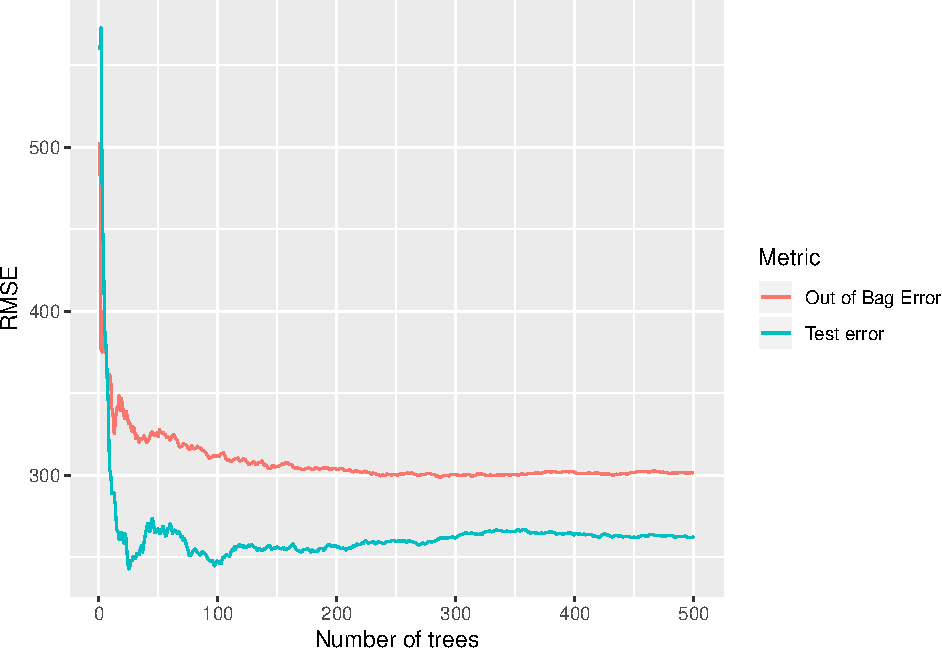
\includegraphics{HW7_files/figure-latex/unnamed-chunk-12-1.pdf}

\subsubsection{Tuning}\label{tuning}

The following is quote from source -
\url{https://uc-r.github.io/random_forests}

\begin{quote}
Random forests are fairly easy to tune since there are only a handful of
tuning parameters. Typically, the primary concern when starting out is
tuning the number of candidate variables to select from at each split.
However, there are a few additional hyperparameters that we should be
aware of. Although the argument names may differ across packages, these
hyperparameters should be present: * ntree: number of trees. We want
enough trees to stabalize the error but using too many trees is
unncessarily inefficient, especially when using large data sets. * mtry:
the number of variables to randomly sample as candidates at each split.
When mtry =p the model equates to bagging. When mtry = 1 the split
variable is completely random, so all variables get a chance but can
lead to overly biased results. A common suggestion is to start with 5
values evenly spaced across the range from 2 to p. * sampsize: the
number of samples to train on. The default value is 63.25\% of the
training set since this is the expected value of unique observations in
the bootstrap sample. Lower sample sizes can reduce the training time
but may introduce more bias than necessary. Increasing the sample size
can increase performance but at the risk of overfitting because it
introduces more variance. Typically, when tuning this parameter we stay
near the 60-80\% range. * nodesize: minimum number of samples within the
terminal nodes. Controls the complexity of the trees. Smaller node size
allows for deeper, more complex trees and smaller node results in
shallower trees. This is another bias-variance tradeoff where deeper
trees introduce more variance (risk of overfitting) and shallower trees
introduce more bias (risk of not fully capturing unique patters and
relatonships in the data). * maxnodes: maximum number of terminal nodes.
Another way to control the complexity of the trees. More nodes equates
to deeper, more complex trees and less nodes result in shallower trees.
\end{quote}

\section{Tuning with H20}\label{tuning-with-h20}

The following code is adapted from the same online source as above. It
will be used to note the most optimal way (effeciency) to tune a random
forest model. I'm using the code as provided by the source because i've
never used the H2o library before and I am very unfamiliary with it's
syntax and operations. It will be used as is in order to come back to as
reference material in the future.

\subsubsection{Start an h2o instance}\label{start-an-h2o-instance}

\begin{Shaded}
\begin{Highlighting}[]
\KeywordTok{h2o.no_progress}\NormalTok{()}
\KeywordTok{h2o.init}\NormalTok{(}\DataTypeTok{max_mem_size =} \StringTok{"5g"}\NormalTok{)}
\end{Highlighting}
\end{Shaded}

\begin{verbatim}
## 
## H2O is not running yet, starting it now...
## 
## Note:  In case of errors look at the following log files:
##     /tmp/RtmpUWlXbI/h2o_scott_started_from_r.out
##     /tmp/RtmpUWlXbI/h2o_scott_started_from_r.err
## 
## 
## Starting H2O JVM and connecting: . Connection successful!
## 
## R is connected to the H2O cluster: 
##     H2O cluster uptime:         1 seconds 151 milliseconds 
##     H2O cluster timezone:       America/Denver 
##     H2O data parsing timezone:  UTC 
##     H2O cluster version:        3.22.1.1 
##     H2O cluster version age:    1 month and 30 days  
##     H2O cluster name:           H2O_started_from_R_scott_sqp085 
##     H2O cluster total nodes:    1 
##     H2O cluster total memory:   4.44 GB 
##     H2O cluster total cores:    8 
##     H2O cluster allowed cores:  8 
##     H2O cluster healthy:        TRUE 
##     H2O Connection ip:          localhost 
##     H2O Connection port:        54321 
##     H2O Connection proxy:       NA 
##     H2O Internal Security:      FALSE 
##     H2O API Extensions:         XGBoost, Algos, AutoML, Core V3, Core V4 
##     R Version:                  R version 3.4.4 (2018-03-15)
\end{verbatim}

\begin{Shaded}
\begin{Highlighting}[]
\CommentTok{# create feature names}
\NormalTok{y <-}\StringTok{ "Crime"}
\NormalTok{x <-}\StringTok{ }\KeywordTok{setdiff}\NormalTok{(}\KeywordTok{names}\NormalTok{(data), y)}

\CommentTok{# turn training set into h2o object}
\NormalTok{train.h2o <-}\StringTok{ }\KeywordTok{as.h2o}\NormalTok{(data)}

\CommentTok{# hyperparameter grid}
\NormalTok{hyper_grid.h2o <-}\StringTok{ }\KeywordTok{list}\NormalTok{(}
  \DataTypeTok{ntrees      =} \KeywordTok{seq}\NormalTok{(}\DecValTok{100}\NormalTok{, }\DecValTok{400}\NormalTok{, }\DataTypeTok{by =} \DecValTok{100}\NormalTok{),}
  \DataTypeTok{mtries      =} \KeywordTok{seq}\NormalTok{(}\DecValTok{2}\NormalTok{, }\DecValTok{10}\NormalTok{, }\DataTypeTok{by =} \DecValTok{2}\NormalTok{),}
  \DataTypeTok{max_depth   =} \KeywordTok{seq}\NormalTok{(}\DecValTok{5}\NormalTok{, }\DecValTok{10}\NormalTok{, }\DataTypeTok{by =} \DecValTok{5}\NormalTok{),}
  \DataTypeTok{min_rows    =} \KeywordTok{seq}\NormalTok{(}\DecValTok{1}\NormalTok{, }\DecValTok{5}\NormalTok{, }\DataTypeTok{by =} \DecValTok{1}\NormalTok{),}
  \DataTypeTok{nbins       =} \KeywordTok{seq}\NormalTok{(}\DecValTok{2}\NormalTok{, }\DecValTok{10}\NormalTok{, }\DataTypeTok{by =} \DecValTok{2}\NormalTok{),}
  \DataTypeTok{sample_rate =} \KeywordTok{c}\NormalTok{(.}\DecValTok{55}\NormalTok{, .}\DecValTok{632}\NormalTok{, .}\DecValTok{75}\NormalTok{)}
\NormalTok{)}

\CommentTok{# random grid search criteria}
\NormalTok{search_criteria <-}\StringTok{ }\KeywordTok{list}\NormalTok{(}
  \DataTypeTok{strategy =} \StringTok{"RandomDiscrete"}\NormalTok{,}
  \DataTypeTok{stopping_metric =} \StringTok{"mse"}\NormalTok{,}
  \DataTypeTok{stopping_tolerance =} \FloatTok{0.005}\NormalTok{,}
  \DataTypeTok{stopping_rounds =} \DecValTok{10}\NormalTok{,}
  \DataTypeTok{max_runtime_secs =} \DecValTok{15}\OperatorTok{*}\DecValTok{60}
\NormalTok{  )}

\CommentTok{# build grid search }
\NormalTok{random_grid <-}\StringTok{ }\KeywordTok{h2o.grid}\NormalTok{(}
  \DataTypeTok{algorithm =} \StringTok{"randomForest"}\NormalTok{,}
  \DataTypeTok{grid_id =} \StringTok{"rf_grid2"}\NormalTok{,}
  \DataTypeTok{x =}\NormalTok{ x, }
  \DataTypeTok{y =}\NormalTok{ y, }
  \DataTypeTok{training_frame =}\NormalTok{ train.h2o,}
  \DataTypeTok{hyper_params =}\NormalTok{ hyper_grid.h2o,}
  \DataTypeTok{search_criteria =}\NormalTok{ search_criteria}
\NormalTok{  )}

\CommentTok{# collect the results and sort by our model performance metric of choice}
\NormalTok{grid_perf2 <-}\StringTok{ }\KeywordTok{h2o.getGrid}\NormalTok{(}
  \DataTypeTok{grid_id =} \StringTok{"rf_grid2"}\NormalTok{, }
  \DataTypeTok{sort_by =} \StringTok{"mse"}\NormalTok{, }
  \DataTypeTok{decreasing =} \OtherTok{FALSE}
\NormalTok{  )}
\KeywordTok{print}\NormalTok{(grid_perf2)}
\end{Highlighting}
\end{Shaded}

\begin{verbatim}
## H2O Grid Details
## ================
## 
## Grid ID: rf_grid2 
## Used hyper parameters: 
##   -  max_depth 
##   -  min_rows 
##   -  mtries 
##   -  nbins 
##   -  ntrees 
##   -  sample_rate 
## Number of models: 1242 
## Number of failed models: 0 
## 
## Hyper-Parameter Search Summary: ordered by increasing mse
##   max_depth min_rows mtries nbins ntrees sample_rate           model_ids
## 1        10      1.0      2     4    300        0.75  rf_grid2_model_357
## 2        10      1.0      2     2    100       0.632  rf_grid2_model_542
## 3        10      1.0      2     8    300       0.632 rf_grid2_model_1155
## 4        10      1.0      4    10    100        0.75  rf_grid2_model_248
## 5         5      2.0      2     6    300        0.75  rf_grid2_model_203
##                  mse
## 1 60697.799275969315
## 2   62245.5339296779
## 3  63505.04913614005
## 4 63997.729454951026
## 5  64162.11313871051
## 
## ---
##      max_depth min_rows mtries nbins ntrees sample_rate
## 1237         5      2.0     10     8    300        0.75
## 1238         5      1.0     10     4    200        0.75
## 1239         5      3.0     10     2    100        0.75
## 1240        10      2.0     10     8    100        0.75
## 1241        10      1.0     10     4    100        0.75
## 1242         5      2.0     10     6    100        0.75
##                model_ids                mse
## 1237 rf_grid2_model_1228  101299.1375502879
## 1238  rf_grid2_model_630 101875.03489284114
## 1239 rf_grid2_model_1127 102255.21642267796
## 1240 rf_grid2_model_1061  102833.4855756525
## 1241  rf_grid2_model_344 107293.71363788348
## 1242  rf_grid2_model_920 109988.34847045377
\end{verbatim}

As we can see above, we ran through 1615 different models to arrive at
the best one. Let's extract the best model using h2o's API, and compare
its RMSE to the original models RMSE of 290.168, at the top of this
section

\begin{Shaded}
\begin{Highlighting}[]
\CommentTok{# Grab the model_id for the top model, chosen by validation error}
\NormalTok{best_model_id <-}\StringTok{ }\NormalTok{grid_perf2}\OperatorTok{@}\NormalTok{model_ids[[}\DecValTok{1}\NormalTok{]]}
\NormalTok{best_model <-}\StringTok{ }\KeywordTok{h2o.getModel}\NormalTok{(best_model_id)}

\CommentTok{# RMSE of best model}
\KeywordTok{h2o.mse}\NormalTok{(best_model) }\OperatorTok\StringTok{ }\KeywordTok{sqrt}\NormalTok{()}
\end{Highlighting}
\end{Shaded}

\begin{verbatim}
## [1] 246.3692
\end{verbatim}

\begin{Shaded}
\begin{Highlighting}[]
\NormalTok{## [1] 23104.67}
\end{Highlighting}
\end{Shaded}

With an RMSE of 242.90, this model is performing better than the non
tuned model. Let's use this model to predict on the new unseen data. We
will compare its results to those of the CART model in the first
section.

\begin{Shaded}
\begin{Highlighting}[]
\NormalTok{pred_h2o <-}\StringTok{ }\KeywordTok{predict}\NormalTok{(best_model, }\KeywordTok{as.h2o}\NormalTok{(new.data))}
\KeywordTok{head}\NormalTok{(pred_h2o)}
\end{Highlighting}
\end{Shaded}

\begin{verbatim}
##   predict
## 1 1115.29
\end{verbatim}

*\textbf{Analysis} The Random Forest model predcited a value of 1172.
This is more along the lines of the values we had been seing in the
other models. Remember that the CART model predict 872. There was a
gross estimation in contrast to all the other models, leading us to the
obvious conlcusion that the Rnadom Forest model is much better than the
simpler CART model

\subsubsection{Always shutdown your h2o instances when
done}\label{always-shutdown-your-h2o-instances-when-done}

\begin{Shaded}
\begin{Highlighting}[]
\KeywordTok{h2o.shutdown}\NormalTok{(}\DataTypeTok{prompt =} \OtherTok{TRUE}\NormalTok{)}
\end{Highlighting}
\end{Shaded}

\begin{verbatim}
## Are you sure you want to shutdown the H2O instance running at http://localhost:54321/ (Y/N)?
\end{verbatim}

\begin{verbatim}
## [1] TRUE
\end{verbatim}

Question 10.2 Describe a situation or problem from your job, everyday
life, current events, etc., for which a logistic regression model would
be appropriate. List some (up to 5) predictors that you might use.

\begin{quote}
Logistic Regression models are used today in the medical field in order
to determine if a patient's tumor is benign or malignant. Various
features can be used in the model to predict one of the binary classes.
Such as: 1. Age of patient 2. Gender 3. Family history with cancer 4.
Length of tumor 5. Width of tumor 6. Any image indicators from CT and/or
Sonograph
\end{quote}

Using the GermanCredit data set germancredit.txt from
\url{http://archive.ics.uci.edu/ml/machine-learning-databases/statlog/german}
/ (description at
\url{http://archive.ics.uci.edu/ml/datasets/Statlog+\%28German+Credit+Data\%29}
), use logistic regression to find a good predictive model for whether
credit applicants are good credit risks or not. Show your model (factors
used and their coefficients), the software output, and the quality of
fit. You can use the glm function in R. To get a logistic regression
(logit) model on data where the response is either zero or one, use
family=binomial(link=''logit'') in your glm function call.

\subsubsection{Load the data}\label{load-the-data}

\begin{Shaded}
\begin{Highlighting}[]
\NormalTok{gc_data <-}\StringTok{ }\KeywordTok{read.table}\NormalTok{(}\StringTok{'germancredit.txt'}\NormalTok{, }\DataTypeTok{header =} \OtherTok{FALSE}\NormalTok{, }\DataTypeTok{stringsAsFactors =} \OtherTok{TRUE}\NormalTok{)}
\NormalTok{gc_data}\OperatorTok{$}\NormalTok{V21 <-}\StringTok{ }\KeywordTok{as.factor}\NormalTok{(gc_data}\OperatorTok{$}\NormalTok{V21)}
\KeywordTok{head}\NormalTok{(gc_data)}
\end{Highlighting}
\end{Shaded}

\begin{verbatim}
##    V1 V2  V3  V4   V5  V6  V7 V8  V9  V10 V11  V12 V13  V14  V15 V16  V17
## 1 A11  6 A34 A43 1169 A65 A75  4 A93 A101   4 A121  67 A143 A152   2 A173
## 2 A12 48 A32 A43 5951 A61 A73  2 A92 A101   2 A121  22 A143 A152   1 A173
## 3 A14 12 A34 A46 2096 A61 A74  2 A93 A101   3 A121  49 A143 A152   1 A172
## 4 A11 42 A32 A42 7882 A61 A74  2 A93 A103   4 A122  45 A143 A153   1 A173
## 5 A11 24 A33 A40 4870 A61 A73  3 A93 A101   4 A124  53 A143 A153   2 A173
## 6 A14 36 A32 A46 9055 A65 A73  2 A93 A101   4 A124  35 A143 A153   1 A172
##   V18  V19  V20 V21
## 1   1 A192 A201   1
## 2   1 A191 A201   2
## 3   2 A191 A201   1
## 4   2 A191 A201   1
## 5   2 A191 A201   2
## 6   2 A192 A201   1
\end{verbatim}

\begin{Shaded}
\begin{Highlighting}[]
\KeywordTok{summary}\NormalTok{(gc_data)}
\end{Highlighting}
\end{Shaded}

\begin{verbatim}
##    V1            V2         V3            V4            V5       
##  A11:274   Min.   : 4.0   A30: 40   A43    :280   Min.   :  250  
##  A12:269   1st Qu.:12.0   A31: 49   A40    :234   1st Qu.: 1366  
##  A13: 63   Median :18.0   A32:530   A42    :181   Median : 2320  
##  A14:394   Mean   :20.9   A33: 88   A41    :103   Mean   : 3271  
##            3rd Qu.:24.0   A34:293   A49    : 97   3rd Qu.: 3972  
##            Max.   :72.0             A46    : 50   Max.   :18424  
##                                     (Other): 55                  
##    V6        V7            V8          V9        V10           V11       
##  A61:603   A71: 62   Min.   :1.000   A91: 50   A101:907   Min.   :1.000  
##  A62:103   A72:172   1st Qu.:2.000   A92:310   A102: 41   1st Qu.:2.000  
##  A63: 63   A73:339   Median :3.000   A93:548   A103: 52   Median :3.000  
##  A64: 48   A74:174   Mean   :2.973   A94: 92              Mean   :2.845  
##  A65:183   A75:253   3rd Qu.:4.000                        3rd Qu.:4.000  
##                      Max.   :4.000                        Max.   :4.000  
##                                                                          
##    V12           V13          V14        V15           V16       
##  A121:282   Min.   :19.00   A141:139   A151:179   Min.   :1.000  
##  A122:232   1st Qu.:27.00   A142: 47   A152:713   1st Qu.:1.000  
##  A123:332   Median :33.00   A143:814   A153:108   Median :1.000  
##  A124:154   Mean   :35.55                         Mean   :1.407  
##             3rd Qu.:42.00                         3rd Qu.:2.000  
##             Max.   :75.00                         Max.   :4.000  
##                                                                  
##    V17           V18          V19        V20      V21    
##  A171: 22   Min.   :1.000   A191:596   A201:963   1:700  
##  A172:200   1st Qu.:1.000   A192:404   A202: 37   2:300  
##  A173:630   Median :1.000                                
##  A174:148   Mean   :1.155                                
##             3rd Qu.:1.000                                
##             Max.   :2.000                                
## 
\end{verbatim}

Looking at the summary of the data, we can see that there is a mix
between numerical columns and categorical columns. We set the
``stringAsFacotrs'' as TRUE. This is R's way of converting string
columns into categorical variables to be handled in the model. For
instances, we can see how R is going to categorize the first column

\begin{Shaded}
\begin{Highlighting}[]
\KeywordTok{contrasts}\NormalTok{(gc_data}\OperatorTok{$}\NormalTok{V1)}
\end{Highlighting}
\end{Shaded}

\begin{verbatim}
##     A12 A13 A14
## A11   0   0   0
## A12   1   0   0
## A13   0   1   0
## A14   0   0   1
\end{verbatim}

We can see that entries of A11 will be encoded as (0,0,0), A12 will be
encoded as (1,0,0), A13 will be encoded as (0,1,0) etc.

\subsubsection{Train / Test Split of
data}\label{train-test-split-of-data}

\begin{Shaded}
\begin{Highlighting}[]
\KeywordTok{set.seed}\NormalTok{(}\DecValTok{42}\NormalTok{)}
\NormalTok{sample =}\StringTok{ }\KeywordTok{sample.split}\NormalTok{(gc_data, }\DataTypeTok{SplitRatio =}\NormalTok{ .}\DecValTok{8}\NormalTok{)}
\NormalTok{train =}\StringTok{ }\KeywordTok{subset}\NormalTok{(gc_data, sample }\OperatorTok{==}\StringTok{ }\OtherTok{TRUE}\NormalTok{)}
\NormalTok{test =}\StringTok{ }\KeywordTok{subset}\NormalTok{(gc_data, sample }\OperatorTok{==}\StringTok{ }\OtherTok{FALSE}\NormalTok{)}
\end{Highlighting}
\end{Shaded}

\subsubsection{Fit the Model}\label{fit-the-model}

\begin{Shaded}
\begin{Highlighting}[]
\NormalTok{gc_model <-}\StringTok{ }\KeywordTok{glm}\NormalTok{(V21 }\OperatorTok{~}\NormalTok{., }\DataTypeTok{family =} \KeywordTok{binomial}\NormalTok{(}\DataTypeTok{link=}\StringTok{'logit'}\NormalTok{), }\DataTypeTok{data =}\NormalTok{ train)}
\KeywordTok{summary}\NormalTok{(gc_model)}
\end{Highlighting}
\end{Shaded}

\begin{verbatim}
## 
## Call:
## glm(formula = V21 ~ ., family = binomial(link = "logit"), data = train)
## 
## Deviance Residuals: 
##     Min       1Q   Median       3Q      Max  
## -2.4184  -0.6750  -0.3459   0.6592   2.5177  
## 
## Coefficients:
##               Estimate Std. Error z value Pr(>|z|)    
## (Intercept)  2.006e+00  1.259e+00   1.593 0.111148    
## V1A12       -2.226e-01  2.583e-01  -0.862 0.388776    
## V1A13       -1.029e+00  4.404e-01  -2.336 0.019480 *  
## V1A14       -1.583e+00  2.750e-01  -5.758 8.49e-09 ***
## V2           3.344e-02  1.105e-02   3.025 0.002485 ** 
## V3A31       -5.816e-01  6.683e-01  -0.870 0.384150    
## V3A32       -1.367e+00  5.352e-01  -2.555 0.010618 *  
## V3A33       -1.544e+00  5.816e-01  -2.655 0.007934 ** 
## V3A34       -2.114e+00  5.486e-01  -3.853 0.000117 ***
## V4A41       -1.812e+00  4.401e-01  -4.118 3.83e-05 ***
## V4A410      -2.171e+00  1.030e+00  -2.107 0.035102 *  
## V4A42       -9.321e-01  3.041e-01  -3.064 0.002180 ** 
## V4A43       -1.196e+00  2.971e-01  -4.028 5.63e-05 ***
## V4A44       -1.494e+01  5.668e+02  -0.026 0.978970    
## V4A45       -2.916e-01  6.728e-01  -0.433 0.664735    
## V4A46       -3.416e-01  4.360e-01  -0.784 0.433248    
## V4A48       -2.032e+00  1.291e+00  -1.574 0.115486    
## V4A49       -1.356e+00  4.025e-01  -3.368 0.000756 ***
## V5           1.277e-04  5.152e-05   2.478 0.013195 *  
## V6A62       -3.780e-01  3.427e-01  -1.103 0.269987    
## V6A63       -2.668e-01  4.490e-01  -0.594 0.552370    
## V6A64       -1.626e+00  6.391e-01  -2.544 0.010954 *  
## V6A65       -1.024e+00  3.075e-01  -3.330 0.000870 ***
## V7A72        1.769e-01  5.172e-01   0.342 0.732308    
## V7A73       -3.159e-01  4.989e-01  -0.633 0.526604    
## V7A74       -6.559e-01  5.264e-01  -1.246 0.212760    
## V7A75       -2.303e-02  5.013e-01  -0.046 0.963362    
## V8           2.814e-01  1.025e-01   2.747 0.006018 ** 
## V9A92       -1.561e-01  4.534e-01  -0.344 0.730539    
## V9A93       -9.241e-01  4.508e-01  -2.050 0.040378 *  
## V9A94       -3.761e-01  5.426e-01  -0.693 0.488209    
## V10A102      4.432e-01  4.788e-01   0.926 0.354555    
## V10A103     -8.265e-01  4.975e-01  -1.661 0.096674 .  
## V11         -3.812e-02  1.028e-01  -0.371 0.710886    
## V12A122      4.635e-02  2.961e-01   0.157 0.875608    
## V12A123     -2.953e-02  2.816e-01  -0.105 0.916496    
## V12A124      6.496e-01  4.957e-01   1.311 0.189962    
## V13         -1.439e-02  1.088e-02  -1.323 0.185806    
## V14A142      1.574e-01  4.757e-01   0.331 0.740787    
## V14A143     -7.768e-01  2.854e-01  -2.722 0.006490 ** 
## V15A152     -5.517e-01  2.773e-01  -1.989 0.046654 *  
## V15A153     -6.840e-01  5.489e-01  -1.246 0.212714    
## V16          1.479e-01  2.221e-01   0.666 0.505403    
## V17A172      5.989e-03  8.008e-01   0.007 0.994033    
## V17A173      8.804e-02  7.682e-01   0.115 0.908756    
## V17A174      1.377e-01  7.722e-01   0.178 0.858504    
## V18          4.943e-01  2.865e-01   1.725 0.084542 .  
## V19A192     -4.104e-01  2.385e-01  -1.720 0.085348 .  
## V20A202     -2.381e+00  1.079e+00  -2.207 0.027345 *  
## ---
## Signif. codes:  0 '***' 0.001 '**' 0.01 '*' 0.05 '.' 0.1 ' ' 1
## 
## (Dispersion parameter for binomial family taken to be 1)
## 
##     Null deviance: 926.51  on 761  degrees of freedom
## Residual deviance: 655.17  on 713  degrees of freedom
## AIC: 753.17
## 
## Number of Fisher Scoring iterations: 14
\end{verbatim}

From the summary above, we can see there are not a lot of features that
are statistically significant. You will also notice that in the data,
there were only 20 features, but in the summary above, there is way more
than 20. This is because the summary function is analyzing every
category for each feature. column V1 had 3 specific categories, and
they're broken out into V1A12, V1A13, V1A14. Also note that the AIC
value is 753.17. Our goal would be to lower this number while improving
the model. A lower value means a better fit. One last note before we
continue on, notice that a lot of the coeffecients are negative. If we
look at a statistically significant value like V1A14 (no checking
account), if you didn't have a checking account, this would reduce your
creditworthiness risk log odds by 1.58

\subsubsection{ANOVA CHI SQUARED TEST}\label{anova-chi-squared-test}

Next we will compare our model to the ``NULL MODEL'' (intercept only
model). By using a chi squared test, we want to see how the deviance in
residuals change as we add each feature one by one. We want to see an
increase in difference between our model and the ``NULL MODEL''

\begin{Shaded}
\begin{Highlighting}[]
\KeywordTok{anova}\NormalTok{(gc_model, }\DataTypeTok{test =} \StringTok{"Chisq"}\NormalTok{)}
\end{Highlighting}
\end{Shaded}

\begin{verbatim}
## Analysis of Deviance Table
## 
## Model: binomial, link: logit
## 
## Response: V21
## 
## Terms added sequentially (first to last)
## 
## 
##      Df Deviance Resid. Df Resid. Dev  Pr(>Chi)    
## NULL                   761     926.51              
## V1    3   97.426       758     829.08 < 2.2e-16 ***
## V2    1   26.138       757     802.94 3.179e-07 ***
## V3    4   26.406       753     776.54 2.621e-05 ***
## V4    9   30.846       744     745.69 0.0003146 ***
## V5    1    0.914       743     744.78 0.3390073    
## V6    4   17.667       739     727.11 0.0014336 ** 
## V7    4   15.419       735     711.69 0.0039061 ** 
## V8    1    4.732       734     706.96 0.0296098 *  
## V9    3   12.828       731     694.13 0.0050234 ** 
## V10   2    4.746       729     689.39 0.0932197 .  
## V11   1    0.020       728     689.37 0.8874504    
## V12   3    2.048       725     687.32 0.5625475    
## V13   1    2.648       724     684.67 0.1036970    
## V14   2   10.605       722     674.07 0.0049787 ** 
## V15   2    3.926       720     670.14 0.1404427    
## V16   1    0.593       719     669.55 0.4414465    
## V17   3    0.190       716     669.36 0.9791643    
## V18   1    3.153       715     666.21 0.0757922 .  
## V19   1    2.497       714     663.71 0.1140365    
## V20   1    8.539       713     655.17 0.0034755 ** 
## ---
## Signif. codes:  0 '***' 0.001 '**' 0.01 '*' 0.05 '.' 0.1 ' ' 1
\end{verbatim}

From the Chi Squared Test, we can see that adding the features V1, V2,
V3, and V4 significantly reduced the Residual Deviance in comparison to
the NULL model, 735 and 926.51 respectively. Adding more features
definetly widens the gap between the NULL model and our model, but the
gap slows down in velocity around V10.

\subsubsection{Model Accuracy}\label{model-accuracy}

\begin{Shaded}
\begin{Highlighting}[]
\NormalTok{test_predict <-}\StringTok{ }\KeywordTok{predict}\NormalTok{(gc_model, }\DataTypeTok{newdata =}\NormalTok{ test[,}\DecValTok{1}\OperatorTok{:}\DecValTok{20}\NormalTok{], }\DataTypeTok{type =}\StringTok{'response'}\NormalTok{)}
\NormalTok{ROC <-}\StringTok{ }\KeywordTok{roc}\NormalTok{(test}\OperatorTok{$}\NormalTok{V21, test_predict)}
\KeywordTok{ggroc}\NormalTok{(ROC) }\OperatorTok{+}\StringTok{ }\KeywordTok{theme_dark}\NormalTok{() }\OperatorTok{+}\StringTok{ }\KeywordTok{ggtitle}\NormalTok{(}\StringTok{'ROC'}\NormalTok{)}
\end{Highlighting}
\end{Shaded}

\includegraphics{HW7_files/figure-latex/unnamed-chunk-23-1.pdf}

\begin{Shaded}
\begin{Highlighting}[]
\KeywordTok{print}\NormalTok{(}\KeywordTok{paste}\NormalTok{(}\StringTok{'AUC: '}\NormalTok{, }\KeywordTok{auc}\NormalTok{(ROC)))}
\end{Highlighting}
\end{Shaded}

\begin{verbatim}
## [1] "AUC:  0.734426499670402"
\end{verbatim}

\begin{Shaded}
\begin{Highlighting}[]
\NormalTok{test_predict <-}\StringTok{ }\KeywordTok{ifelse}\NormalTok{(test_predict }\OperatorTok{>}\StringTok{ }\FloatTok{0.20}\NormalTok{, }\DecValTok{2}\NormalTok{, }\DecValTok{1}\NormalTok{)}
\KeywordTok{confusionMatrix}\NormalTok{(}\KeywordTok{as.factor}\NormalTok{(test_predict), }\KeywordTok{as.factor}\NormalTok{(test}\OperatorTok{$}\NormalTok{V21), }\DataTypeTok{positive =} \StringTok{'2'}\NormalTok{)}
\end{Highlighting}
\end{Shaded}

\begin{verbatim}
## Confusion Matrix and Statistics
## 
##           Reference
## Prediction  1  2
##          1 99 22
##          2 65 52
##                                           
##                Accuracy : 0.6345          
##                  95% CI : (0.5698, 0.6957)
##     No Information Rate : 0.6891          
##     P-Value [Acc > NIR] : 0.9693          
##                                           
##                   Kappa : 0.2642          
##  Mcnemar's Test P-Value : 6.704e-06       
##                                           
##             Sensitivity : 0.7027          
##             Specificity : 0.6037          
##          Pos Pred Value : 0.4444          
##          Neg Pred Value : 0.8182          
##              Prevalence : 0.3109          
##          Detection Rate : 0.2185          
##    Detection Prevalence : 0.4916          
##       Balanced Accuracy : 0.6532          
##                                           
##        'Positive' Class : 2               
## 
\end{verbatim}

From our ``all features'' model, we can see that we got about 76\%
Accuracy using a 50\% logit prediction model (meaning if a prediction
was greater than 0.5, then 2, if it is 0.5 or less, then 1). Let's now
try to tune our model and also tune the prediction threshold.

\subsubsection{Tuning}\label{tuning-1}

From our Chi Square test results, let's use the most statitically
significant features from that test.

\begin{enumerate}
\def\labelenumi{\arabic{enumi}.}
\tightlist
\item
  V1 - Status of existing checking
\item
  V2 - Duration in month
\item
  V3 - Credit History
\item
  V4 - Purpose
\item
  V6 - Savings Account balance
\item
  V7 - Present Employment
\item
  V9 - Personal Status and Sex
\item
  V14 - Other installment plans
\item
  V20 - Foreign Worker
\end{enumerate}

\begin{Shaded}
\begin{Highlighting}[]
\NormalTok{train_final <-}\StringTok{ }\NormalTok{train[, }\KeywordTok{c}\NormalTok{(}\DecValTok{1}\NormalTok{,}\DecValTok{2}\NormalTok{,}\DecValTok{3}\NormalTok{,}\DecValTok{4}\NormalTok{,}\DecValTok{6}\NormalTok{,}\DecValTok{7}\NormalTok{,}\DecValTok{9}\NormalTok{,}\DecValTok{14}\NormalTok{,}\DecValTok{20}\NormalTok{,}\DecValTok{21}\NormalTok{)]}
\NormalTok{test_final <-}\StringTok{ }\NormalTok{test[, }\KeywordTok{c}\NormalTok{(}\DecValTok{1}\NormalTok{,}\DecValTok{2}\NormalTok{,}\DecValTok{3}\NormalTok{,}\DecValTok{4}\NormalTok{,}\DecValTok{6}\NormalTok{,}\DecValTok{7}\NormalTok{,}\DecValTok{9}\NormalTok{,}\DecValTok{14}\NormalTok{,}\DecValTok{20}\NormalTok{,}\DecValTok{21}\NormalTok{)]}

\NormalTok{final_model <-}\StringTok{ }\KeywordTok{glm}\NormalTok{(V21 }\OperatorTok{~}\NormalTok{., }\DataTypeTok{family =} \KeywordTok{binomial}\NormalTok{(}\DataTypeTok{link=}\StringTok{'logit'}\NormalTok{), }\DataTypeTok{data =}\NormalTok{ train_final)}



\NormalTok{final_predict <-}\StringTok{ }\KeywordTok{predict}\NormalTok{(final_model, }\DataTypeTok{newdata =}\NormalTok{ test_final, }\DataTypeTok{type =}\StringTok{'response'}\NormalTok{)}
\NormalTok{final_ROC <-}\StringTok{ }\KeywordTok{roc}\NormalTok{(test_final}\OperatorTok{$}\NormalTok{V21, final_predict)}
\KeywordTok{ggroc}\NormalTok{(final_ROC) }\OperatorTok{+}\StringTok{ }\KeywordTok{theme_dark}\NormalTok{() }\OperatorTok{+}\StringTok{ }\KeywordTok{ggtitle}\NormalTok{(}\StringTok{'ROC'}\NormalTok{)}
\end{Highlighting}
\end{Shaded}

\includegraphics{HW7_files/figure-latex/unnamed-chunk-24-1.pdf}

\begin{Shaded}
\begin{Highlighting}[]
\KeywordTok{print}\NormalTok{(}\KeywordTok{paste}\NormalTok{(}\StringTok{'AUC: '}\NormalTok{, }\KeywordTok{auc}\NormalTok{(ROC)))}
\end{Highlighting}
\end{Shaded}

\begin{verbatim}
## [1] "AUC:  0.734426499670402"
\end{verbatim}

\begin{Shaded}
\begin{Highlighting}[]
\NormalTok{final_predict <-}\StringTok{ }\KeywordTok{ifelse}\NormalTok{(final_predict }\OperatorTok{>}\StringTok{ }\FloatTok{0.15}\NormalTok{, }\DecValTok{2}\NormalTok{, }\DecValTok{1}\NormalTok{)}
\KeywordTok{confusionMatrix}\NormalTok{(}\KeywordTok{as.factor}\NormalTok{(final_predict), }\KeywordTok{as.factor}\NormalTok{(test_final}\OperatorTok{$}\NormalTok{V21), }\DataTypeTok{positive =} \StringTok{'2'}\NormalTok{)}
\end{Highlighting}
\end{Shaded}

\begin{verbatim}
## Confusion Matrix and Statistics
## 
##           Reference
## Prediction  1  2
##          1 85 17
##          2 79 57
##                                           
##                Accuracy : 0.5966          
##                  95% CI : (0.5313, 0.6595)
##     No Information Rate : 0.6891          
##     P-Value [Acc > NIR] : 0.999           
##                                           
##                   Kappa : 0.2346          
##  Mcnemar's Test P-Value : 4.791e-10       
##                                           
##             Sensitivity : 0.7703          
##             Specificity : 0.5183          
##          Pos Pred Value : 0.4191          
##          Neg Pred Value : 0.8333          
##              Prevalence : 0.3109          
##          Detection Rate : 0.2395          
##    Detection Prevalence : 0.5714          
##       Balanced Accuracy : 0.6443          
##                                           
##        'Positive' Class : 2               
## 
\end{verbatim}

Conclusion: After playing around with several probability thresholds,
with the ``tuned'' model, it still couldn't quite get to the results of
the all variables model. Therefore, we will express the answer in terms
of the all variables model

\subsubsection{Model Coeficients}\label{model-coeficients}

\begin{Shaded}
\begin{Highlighting}[]
\NormalTok{coef =}\StringTok{ }\KeywordTok{as.matrix}\NormalTok{(gc_model}\OperatorTok{$}\NormalTok{coefficients)}
\NormalTok{coef}
\end{Highlighting}
\end{Shaded}

\begin{verbatim}
##                      [,1]
## (Intercept)  2.005960e+00
## V1A12       -2.226314e-01
## V1A13       -1.028931e+00
## V1A14       -1.583297e+00
## V2           3.343583e-02
## V3A31       -5.816336e-01
## V3A32       -1.367420e+00
## V3A33       -1.544016e+00
## V3A34       -2.113856e+00
## V4A41       -1.811993e+00
## V4A410      -2.171294e+00
## V4A42       -9.320606e-01
## V4A43       -1.196399e+00
## V4A44       -1.494222e+01
## V4A45       -2.916034e-01
## V4A46       -3.416328e-01
## V4A48       -2.031583e+00
## V4A49       -1.355907e+00
## V5           1.276948e-04
## V6A62       -3.779772e-01
## V6A63       -2.667757e-01
## V6A64       -1.626021e+00
## V6A65       -1.023886e+00
## V7A72        1.768956e-01
## V7A73       -3.159155e-01
## V7A74       -6.558751e-01
## V7A75       -2.302906e-02
## V8           2.814237e-01
## V9A92       -1.561413e-01
## V9A93       -9.240783e-01
## V9A94       -3.760751e-01
## V10A102      4.432319e-01
## V10A103     -8.264608e-01
## V11         -3.811712e-02
## V12A122      4.634545e-02
## V12A123     -2.952799e-02
## V12A124      6.496454e-01
## V13         -1.439163e-02
## V14A142      1.573682e-01
## V14A143     -7.768228e-01
## V15A152     -5.517392e-01
## V15A153     -6.840414e-01
## V16          1.479307e-01
## V17A172      5.988959e-03
## V17A173      8.804191e-02
## V17A174      1.376658e-01
## V18          4.942606e-01
## V19A192     -4.103831e-01
## V20A202     -2.380572e+00
\end{verbatim}

\subsubsection{Probablility Threshold}\label{probablility-threshold}

\begin{Shaded}
\begin{Highlighting}[]
\NormalTok{cm <-}\StringTok{ }\KeywordTok{confusionMatrix}\NormalTok{(}\KeywordTok{as.factor}\NormalTok{(test_predict), }\KeywordTok{as.factor}\NormalTok{(test}\OperatorTok{$}\NormalTok{V21), }\DataTypeTok{positive =} \StringTok{'2'}\NormalTok{)}
\NormalTok{cm}\OperatorTok{$}\NormalTok{table}
\end{Highlighting}
\end{Shaded}

\begin{verbatim}
##           Reference
## Prediction  1  2
##          1 99 22
##          2 65 52
\end{verbatim}

A threshold of 20\% gave the best results of limiting the 5x damage of
incorrectly predicting a ``bad credit risk''


\end{document}
